%! Author = joels
%! Date = 24/12/2020

\section{Standard Container \& Iterators}
% You know the properties of the different standard containers
% You can select the best standard containers for your application
% You know the different iterator categories and their capabilities
% You can explain the difference between a const iterator and a const_iterator

\subsection{STL Containers: General API}
\begin{itemize}
    \item Sequence Containers
        \SubItem{Elements are accessible in order as they were inserted created}
        \SubItem{Find in linear time through the algorithm find}
    \item Associative Containers
        \SubItem{Elements are accessible in sorted order}
        \SubItem{find as member function in logarithmic time}
    \item Hashed Containers
        \SubItem{Elements are accessible in unspecified order}
        \SubItem{find as member function in constant time}
\end{itemize}
\begin{center}
    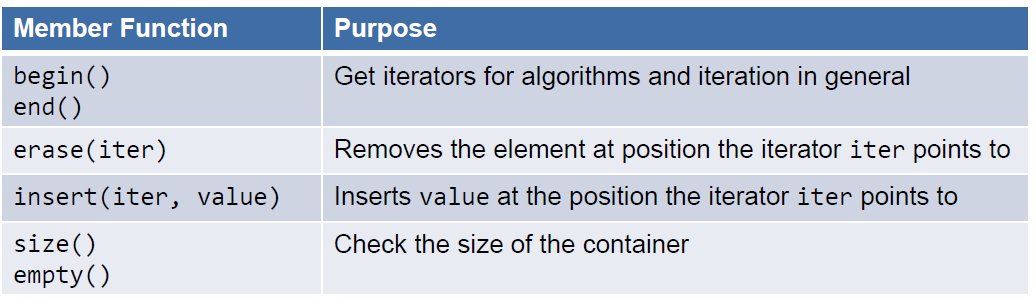
\includegraphics[scale=0.45]{container_functions.png}
\end{center}

\subsection{Sequence Containers}
\subsubsection{std::vector \& std::array}
Siehe Kapitel3: Sequences and Iterators (Seite 6)
\subsubsection{std::deque$<$T$>$ $\rightarrow$ \#include$<$deque$>$}
std::deque is like std::vector but with additional, efficient front insertion/removal
\begin{center}
    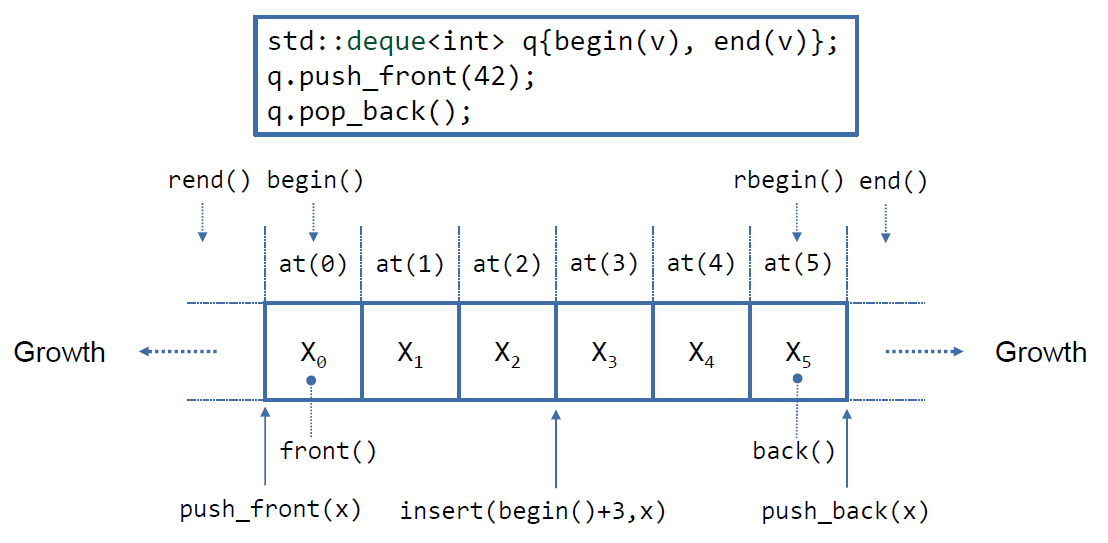
\includegraphics[scale=0.43]{deque.png}
\end{center}
\subsubsection{std::list$<$T$>$ $\rightarrow$ \#include$<$list$>$}
Efficient insertion in any position. Lower efficiency in bulk operations. Requires member function call for sort etc. Only bi directional iterators no index access
\begin{center}
    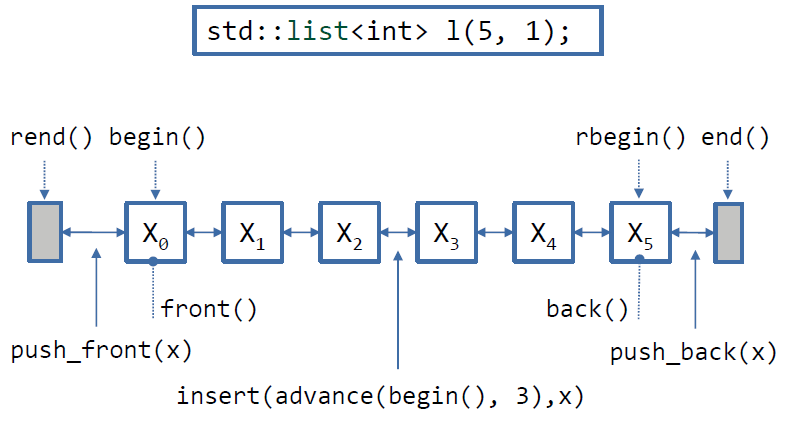
\includegraphics[scale=0.43]{list.png}
\end{center}
\subsubsection{std::forward\_list$<$T$>$ $\rightarrow$ \#include$<$forward\_list$>$}
Efficient insertion AFTER any position, but clumsy with iterator to get \dq before\dq position. Only forward iterators, clumsy to search and remove, use member functions not algorithms.
\begin{center}
    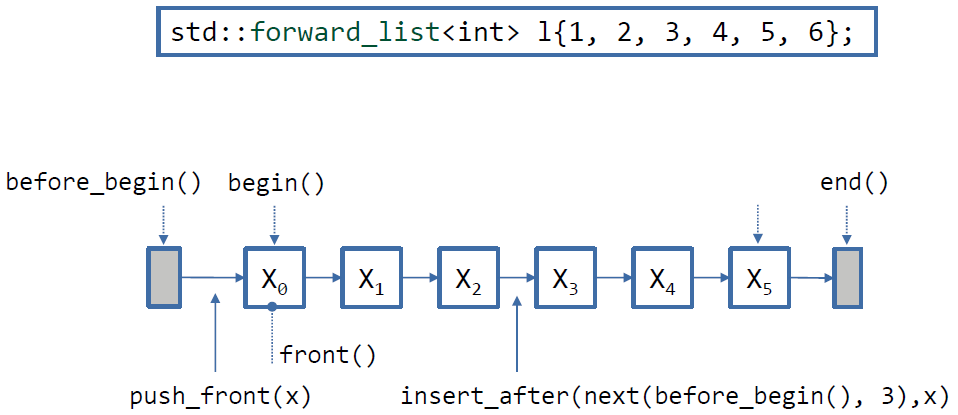
\includegraphics[scale=0.45]{forward_list}
\end{center}
\subsubsection{std::stack $\rightarrow$ \#include$<$stack$>$}
Uses std::deque (or std::vector, std::list) and limits its functionality to stack operations. Iteration not possible.
\begin{center}
    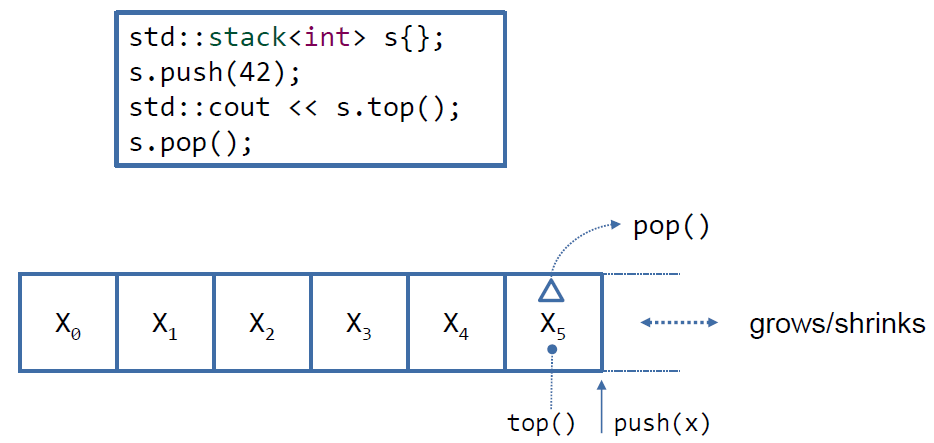
\includegraphics[scale=0.45]{stack.png}
\end{center}
\subsubsection{std::queue $\rightarrow$ \#include$<$queue$>$}
Uses std::deque (or std::list) and limits its functionality to queue operations. Iteration not possible.
\begin{center}
    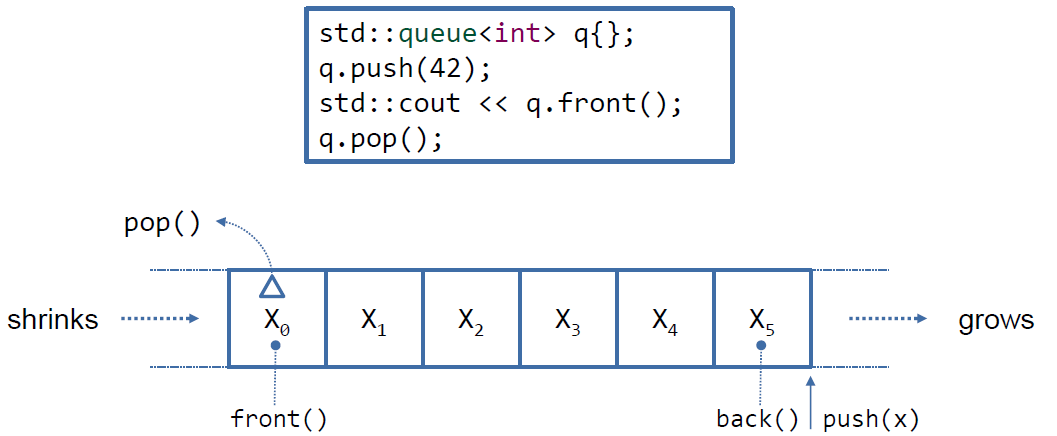
\includegraphics[scale=0.45]{queue.png}
\end{center}
\subsubsection{std::priority\_queue $\rightarrow$ \#include$<$stack$>$}
Uses std::deque (or std::vector) and limits its functionality to stack operations. top() element is always the smallest.
\begin{center}
    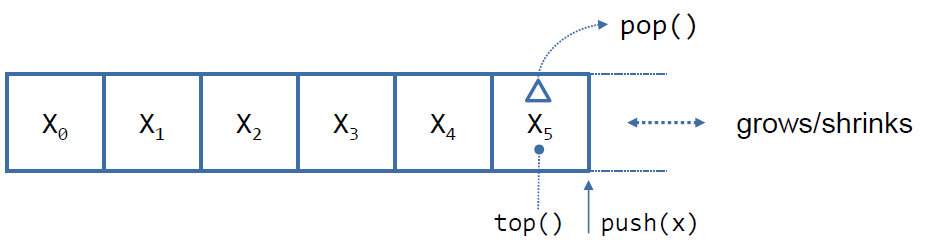
\includegraphics[scale=0.45]{priority_queue.png}
\end{center}
\subsection{Associative Containers}

\subsubsection{std::set}

\subsubsection{std::map}

\subsubsection{std::multiset}

\subsection{Hashed Containers}

\subsubsection{std::unordered\_set}

\subsubsection{std::unordered\_map}

\subsection{Iterators}

\subsubsection{Input Iterator}

\subsubsection{Forward Iterator}

\subsubsection{Bidirectional Iterator}

\subsubsection{Random Access Iterator}

\subsubsection{Output Iterator}

\subsubsection{Iterator Functions}

\subsubsection{std::advance vs. std::next}